\begin{figure}[htbp]
\centering
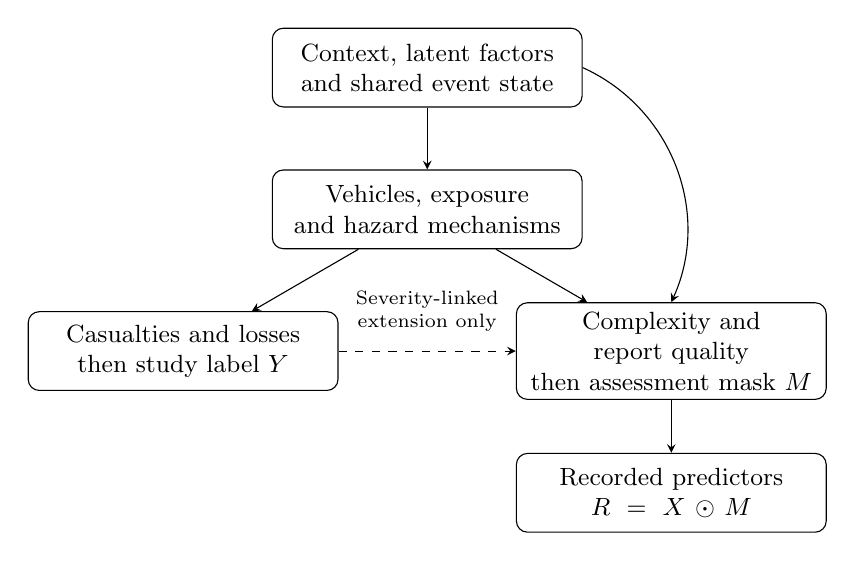
\begin{tikzpicture}[every node/.style={draw,rounded corners,align=center,font=\small,text width=3.7cm,minimum height=1cm},>=stealth]
\node (event) at (0,3.6) {Context, latent factors\\and shared event state};
\node (physical) at (0,1.8) {Vehicles, exposure\\and hazard mechanisms};
\node (outcome) at (-3.1,0) {Casualties and losses\\then study label $Y$};
\node (mask) at (3.1,0) {Complexity and report quality\\then assessment mask $M$};
\node (features) at (3.1,-1.8) {Recorded predictors\\$R=X\odot M$};
\draw[->] (event)--(physical);
\draw[->] (physical)--(outcome);
\draw[->] (physical)--(mask);
\draw[->] (event.east) to[bend left=45] (mask.north);
\draw[->] (mask)--(features);
\draw[->,dashed] (outcome)-- node[above,draw=none,text width=2cm,font=\scriptsize] {Severity-linked\\extension only} (mask);
\end{tikzpicture}
\caption{Schematic of the declared generating mechanism. The primary mask receives shared event complexity but no casualty or loss field. The dashed connection is added only in the severity-linked recording intervention. Models receive $R$; outcome fields and diagnostic masks are excluded from primary predictors.}
\label{fig:process}
\end{figure}